\documentclass[12pt,twoside]{article}

\textwidth 17cm \textheight 25cm \evensidemargin 0cm
\oddsidemargin 0cm \topmargin -2cm
\parindent 0pt
%\parskip \bigskipamount

\usepackage{graphicx}
\usepackage[dutch]{babel}
\usepackage{amssymb,amsthm,amsmath}
%\usepackage{dot2texi}
\usepackage[utf8]{inputenc}
\usepackage{nopageno}
\usepackage{pdfpages}
\usepackage{enumerate}
\usepackage{caption}
\usepackage{wrapfig}
\usepackage{pgf,tikz,pgfplots}
\pgfplotsset{compat=1.15}
\usepackage{color}
\usetikzlibrary{arrows}
\usetikzlibrary{patterns}
\usepackage{fancyhdr}
\pagestyle{fancy}
\usepackage[version=3]{mhchem}
\usepackage{multicol}
\usepackage{fix-cm}
\usepackage{setspace}
\usepackage{mhchem}
\usepackage{xhfill}
\usepackage{parskip}
\usepackage{cancel}
\usepackage{mdframed}
\usepackage{url}
\usepackage{mathtools}
\usepackage{changepage}

\newcommand{\todo}[1]{{\color{red} TODO: #1}}

\newcommand{\degree}{\ensuremath{^\circ}}
\newcommand\rad{\qopname\relax o{\mathrm{rad}}}

\newcommand\ggd{\qopname\relax o{\mathrm{ggd}}}

\pgfmathdeclarefunction{gauss}{2}{%
  \pgfmathparse{1/(#2*sqrt(2*pi))*exp(-((x-#1)^2)/(2*#2^2))}%
}

\def\LRA{\Leftrightarrow}

\newcommand{\zrmbox}{\framebox{\phantom{EXE}}\phantom{X}}
\newcommand{\zrm}[1]{\framebox{#1}}

% environment oefening:
% houdt een teller bij die de oefeningen nummert, probeert ook de oefening op één pagina te houden
\newcounter{noefening}
\setcounter{noefening}{0}
\newenvironment{oefening}
{
  \stepcounter{noefening}
  \pagebreak[0]
  \begin{minipage}{\textwidth}
  \vspace*{0.7cm}{\large\bf Oefening \arabic{noefening}}
}{%
  \end{minipage}
}

\usepackage{calc}

% vraag
\reversemarginpar
\newcounter{punten}
\setcounter{punten}{0}
\newcounter{nvraag}
\setcounter{nvraag}{1}
\newlength{\puntwidth}
\newlength{\boxwidth}
\newcommand{\vraag}[1]{
\settowidth{\puntwidth}{\Large{#1}}
\setlength{\boxwidth}{1.5cm}
\addtolength{\boxwidth}{-\puntwidth}
{\large\bf Vraag \arabic{nvraag} \addtocounter{nvraag}{1}}\vspace*{-0.5cm}
{\marginpar{\color{lightgray}\fbox{\parbox{1.5cm}{\vspace*{1cm}\hspace*{\boxwidth}{\Large{#1}}}}}
\vspace*{0.5cm}}
\addtocounter{punten}{#1}}

% arulefill
\def\arulefill{\leavevmode{\xrfill[-5pt]{0.3pt}[lightgray]\endgraf}\vspace*{0.2cm}}

% \arules{n}
\newcommand{\arules}[1]{
\color{lightgray}
%\vspace*{0.05cm}
\foreach \n in {1,...,#1}{
  \vspace*{0.75cm}
  \hrule height 0.3pt\hfill
}\color{black}\vspace*{0.2cm}}

% \arule{x}
\newcommand{\arule}[1]{
\color{lightgray}{\raisebox{-0.1cm}{\rule[-0.05cm]{#1}{0.3pt}}}\color{black}
}

% \abox{y}
\newcommand{\abox}[1]{
\fbox{
\begin{minipage}{\textwidth- 4\fboxsep}
\hspace*{\textwidth}\vspace{#1}
\end{minipage}
}
}

\newcommand{\ruitjes}[1]{
\definecolor{cqcqcq}{rgb}{0.85,0.85,0.85}
\hspace*{-2.5cm}
\begin{tikzpicture}[scale=1.04,line cap=round,line join=round,>=triangle 45,x=1.0cm,y=1.0cm]
\draw [color=cqcqcq, xstep=0.5cm, ystep=0.5cm] (0,-#1) grid (20.5,0);
\end{tikzpicture}
}


\newcommand{\assenstelsel}[5][1]{
\definecolor{cqcqcq}{rgb}{0.65,0.65,0.65}
\begin{tikzpicture}[line cap=round,line join=round,>=triangle 45,x=#1cm,y=#1cm]
\draw [color=cqcqcq,dash pattern=on 1pt off 1pt, xstep=1.0cm,ystep=1.0cm] (#2,#4) grid (#3,#5);
\draw[->,color=black] (#2,0) -- (#3,0);
%\draw[shift={(1,0)},color=black] (0pt,2pt) -- (0pt,-2pt) node[below] {\footnotesize $1$};
%\draw[color=black] (#3.25,0.07) node [anchor=south west] {$x$};
\draw[->,color=black] (0,#4) -- (0,#5);
%\draw[shift={(0,1)},color=black] (2pt,0pt) -- (-2pt,0pt) node[left] {\footnotesize $1$};
\draw[color=black] (0.09,#5.25) node [anchor=west] {\phantom{$y$}};
%\draw[color=black] (0pt,-10pt) node[right] {\footnotesize $0$};
\end{tikzpicture}
}

\newcommand{\getallenas}[3][1]{
\definecolor{cqcqcq}{rgb}{0.65,0.65,0.65}
\begin{tikzpicture}[scale=#1,line cap=round,line join=round,>=triangle 45,x=1.0cm,y=1.0cm]
\draw [color=cqcqcq,dash pattern=on 1pt off 1pt, xstep=1.0cm,ystep=1.0cm] (#2,-0.2) grid (#3,0.2);
\draw[->,color=black] (#2.25,0) -- (#3.5,0);
\draw[shift={(0,0)},color=black] (0pt,2pt) -- (0pt,-2pt) node[below] {\footnotesize $0$};
\draw[shift={(1,0)},color=black] (0pt,2pt) -- (0pt,-2pt) node[below] {\footnotesize $1$};
\draw[color=black] (#3.25,0.07) node [anchor=south west] {$\mathbb{R}$};
\end{tikzpicture}
}

\newcommand{\visgraad}[1]{\begin{tabular}{p{0.5cm}|p{#1}}&\\\hline\\\end{tabular}}

\newcommand{\tekenschema}[2]{\begin{tabular}{p{0.5cm}|p{#1}}&\\\hline\\[#2]\end{tabular}}

% schema van Horner
\newcommand{\schemahorner}{
\begin{tabular}{p{0.5cm}|p{7cm}}
&\\[1.5cm]
\hline\\
\end{tabular}}

% geef tabular iets meer ruimte
\setlength{\tabcolsep}{14pt}
\renewcommand{\arraystretch}{1.5}

\newcommand{\toets}[3]{
\thispagestyle{plain}
\vspace*{-2.5cm}
\begin{tikzpicture}[remember picture, overlay]
    \node [shift={(15.25 cm,-1.6cm)}] {%
        \includegraphics[width=1.8cm]{/home/ppareit/kaa1415/logokaavelgem.png}%
    };%
\end{tikzpicture}

\begin{tabular}{|llc|c|}
\hline
\vspace*{-0.5cm}
&&&\\
Naam & \arule{4cm} & {\Large\bf KA AVELGEM} & \\
\vspace*{-0.75cm}
&&&\\
Klas & \arule{4cm} & {\Large\bf 20...-...-...} & \\
\hline
\vspace*{-0.75cm}
&&&\\
Toets & {\bf #2} & {\large\bf #1} & Beoordeling\\
\vspace*{-0.75cm}
&&&\\
Onderwerp & \multicolumn{2}{l|}{\bf #3} &\\
\hline
\end{tabular}
}

\newcommand{\oefeningen}[1]{

\fancyhead[LE, RO]{\vspace{0.5cm} #1}
%\thispagestyle{plain}

{\bf \Large \centering Oefeningen: #1}

}

\raggedbottom

\newcommand\vl{\qopname\relax o{\mathrm{vl}}}

\newcommand\dom{\qopname\relax o{\mathrm{dom}}}
\newcommand\ber{\qopname\relax o{\mathrm{ber}}}

\newcommand\mC{\qopname\relax o{\mathrm{mC}}}
\newcommand\uC{\qopname\relax o{\mathrm{{\mu}C}}}
\newcommand\C{\qopname\relax o{\mathrm{C}}}

\newcommand\W{\qopname\relax o{\mathrm{W}}}
\newcommand\kW{\qopname\relax o{\mathrm{kW}}}
\newcommand\kWh{\qopname\relax o{\mathrm{kWh}}}


\newcommand\V{\qopname\relax o{\mathrm{V}}}
\newcommand\ohm{\qopname\relax o{\mathrm{\Omega}}}
\newcommand\kohm{\qopname\relax o{\mathrm{k\Omega}}}


\newcommand\N{\qopname\relax o{\mathrm{N}}}

\newcommand\Nperkg{\qopname\relax o{\mathrm{N/kg}}}

\newcommand\Nperm{\qopname\relax o{\mathrm{N/m}}}

\newcommand\gpermol{\qopname\relax o{\mathrm{g/mol}}}


\newcommand\kgperm{\qopname\relax o{\mathrm{kg/m}}}
\newcommand\kgperdm{\qopname\relax o{\mathrm{kg/dm}}}
\newcommand\gpercm{\qopname\relax o{\mathrm{g/cm}}}
\newcommand\gperml{\qopname\relax o{\mathrm{g/ml}}}


\newcommand{\mA}{\;\mbox{mA}}
\newcommand{\A}{\;\mbox{A}}
\newcommand{\MA}{\;\mbox{MA}}

\newcommand{\us}{\;\mu\mbox{s}}
\newcommand\s{\qopname\relax o{\mathrm{s}}}

\newcommand\h{\qopname\relax o{\mathrm{h}}}

\newcommand{\kmperh}{\;\mbox{km/h}}
\newcommand{\mpers}{\;\mbox{m/s}}
\newcommand{\kmpermin}{\;\mbox{km/min}}
\newcommand{\kmpers}{\;\mbox{km/s}}

\newcommand{\mph}{\;\mbox{mph}}

\newcommand{\Hz}{\;\mbox{Hz}}

\newcommand\Gm{\qopname\relax o{\mathrm{Gm}}}
\newcommand\Mm{\qopname\relax o{\mathrm{Mm}}}
\newcommand\km{\qopname\relax o{\mathrm{km}}}
\newcommand\hm{\qopname\relax o{\mathrm{hm}}}
\newcommand\dam{\qopname\relax o{\mathrm{dam}}}
\newcommand\m{\qopname\relax o{\mathrm{m}}}
\newcommand\dm{\qopname\relax o{\mathrm{dm}}}
\newcommand\cm{\qopname\relax o{\mathrm{cm}}}
\newcommand\mm{\qopname\relax o{\mathrm{mm}}}
\newcommand\um{\qopname\relax o{\mathrm{{\mu}m}}}
\newcommand\nm{\qopname\relax o{\mathrm{nm}}}


\newcommand\Gg{\qopname\relax o{\mathrm{Gg}}}
\newcommand\Mg{\qopname\relax o{\mathrm{Mg}}}
\newcommand\kg{\qopname\relax o{\mathrm{kg}}}
\newcommand\hg{\qopname\relax o{\mathrm{hg}}}
\renewcommand\dag{\qopname\relax o{\mathrm{dag}}}
\newcommand\g{\qopname\relax o{\mathrm{g}}}
\newcommand\dg{\qopname\relax o{\mathrm{dg}}}
\newcommand\cg{\qopname\relax o{\mathrm{cg}}}
\newcommand\mg{\qopname\relax o{\mathrm{mg}}}
\newcommand\ug{\qopname\relax o{\mathrm{{\mu}g}}}
\renewcommand\ng{\qopname\relax o{\mathrm{ng}}}

\newcommand\ton{\qopname\relax o{\mathrm{ton}}}

\newcommand\Gl{\qopname\relax o{\mathrm{Gl}}}
\newcommand\Ml{\qopname\relax o{\mathrm{Ml}}}
\newcommand\kl{\qopname\relax o{\mathrm{kl}}}
\newcommand\hl{\qopname\relax o{\mathrm{hl}}}
\newcommand\dal{\qopname\relax o{\mathrm{dal}}}
\renewcommand\l{\qopname\relax o{\mathrm{l}}}
\newcommand\dl{\qopname\relax o{\mathrm{dl}}}
\newcommand\cl{\qopname\relax o{\mathrm{cl}}}
\newcommand\ml{\qopname\relax o{\mathrm{ml}}}
\newcommand\ul{\qopname\relax o{\mathrm{{\mu}l}}}
\newcommand\nl{\qopname\relax o{\mathrm{nl}}}

\newcommand\MJ{\qopname\relax o{\mathrm{MJ}}}
\newcommand\kJ{\qopname\relax o{\mathrm{kJ}}}
\newcommand\J{\qopname\relax o{\mathrm{J}}}

\newcommand\T{\qopname\relax o{\mathrm{T}}}
\newcommand\uT{\qopname\relax o{\mathrm{{\mu}T}}}

\newcommand\grC{\qopname\relax o{\mathrm{{\degree}C}}}

\newcommand\K{\qopname\relax o{\mathrm{K}}}
\newcommand\calperK{\qopname\relax o{\mathrm{cal/K}}}

\newcommand\hPa{\qopname\relax o{\mathrm{hPa}}}
\newcommand\Pa{\qopname\relax o{\mathrm{Pa}}}

\newcommand\dB{\qopname\relax o{\mathrm{dB}}}

\newcommand\Var{\qopname\relax o{\mathrm{Var}}}

\newcommand{\EE}[1]{\cdot 10^{#1}}

\onehalfspacing

%\setlength{\headsep}{0cm}

\newenvironment{exlist}[1] %
{ \begin{multicols}{#1}
  \begin{enumerate}[(a)]
    \setlength{\itemsep}{0.5em} }
{ \end{enumerate}
  \end{multicols} }




%\renewcommand{\rmdefault}{phv} % Arial
%\renewcommand{\sfdefault}{phv} % Arial

\newcommand{\dice}[1]{
\begin{tikzpicture}[x=1em,y=1em,radius=0.1]
  \draw[rounded corners=1] (0,0) rectangle (1,1);
  \ifodd#1
    \fill (0.5,0.5) circle;
  \fi
  \ifnum#1>1
    \fill (0.2,0.2) circle;
    \fill (0.8,0.8) circle;
   \ifnum#1>3
     \fill (0.2,0.8) circle;
     \fill (0.8,0.2) circle;
    \ifnum#1>5
      \fill (0.8,0.5) circle;
      \fill (0.2,0.5) circle;
    \fi
  \fi
\fi
\end{tikzpicture}
}

\begin{document}

\thispagestyle{empty}
\begin{center}
  \begin{mdframed}
  \centering
  \fontsize{40}{60}\selectfont Elementaire kansrekening
  \end{mdframed}
  %\vfill
  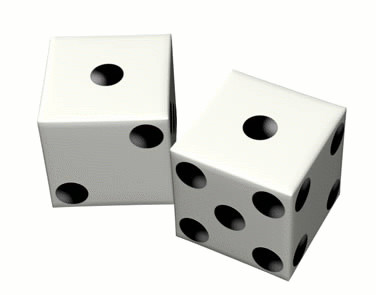
\includegraphics[width=0.8\textwidth]{dice}
  %\vfill
\end{center}
%\vfill
\vspace*{-3cm}
\subsection*{Doelstellingen}
{\singlespacing
Je kan \hfill  {\scriptsize(LP 2006-059, LI 2.2)}
\begin{itemize}
  \item de begrippen kansexperiment, uitkomst en gebeurtenis in een toepassing onderscheiden
  \item de regel van Laplace, de somregel en de complementregel bij het oplossen van oefeningen toepassen
  \item het onderscheid maken tussen een gewone kans en een voorwaardelijke kans
  \item een voorwaardelijke kans bepalen
  \item bepalen of twee gebeurtenissen al dan niet statistisch afhankelijk zijn
  \item besluiten trekken in verband met statistische afhankelijkheid bij trekkingen met en zonder terugleggen
\end{itemize}}
\subsection*{Algemene vaardigheden en attitudes}
{\singlespacing
Je \hfill {\scriptsize(LP 2006/059, ET1, ET9, ET11)}
\begin{itemize}
  \itemsep0em
  \item begrijpt en gebruikt wiskundetaal.
  \item gebruikt kennis, inzicht en vaardigheden die je verwerft in de wiskunde bij het verkennen, vertolken en verklaren van problemen uit de realiteit.
  \item ontwikkelt zelfregulatie met betrekking tot het verwerven en verwerken van wiskundige informatie en het oplossen van problemen
\end{itemize}
}
\vspace*{-2cm}

\thispagestyle{empty}
\mbox{}
\newpage
\clearpage
\thispagestyle{empty}
\mbox{}
\newpage
\clearpage
\pagenumbering{arabic} 

\fancyhead[RO,LE]{Elementaire kansrekening}
\fancyhead[RE,LO]{}

\section{Inleiding}

\begin{oefening}
Ga voor volgende problemen na of je de kans zou kunnen berekenen of je ze enkel kan schatten.
\begin{enumerate}[(a)]
  \item Hoe groot is de kans dat het in België in de maand januari 5 opeenvolgende nachten vriest?
  \arules{3}
  \item Hoe groot is de kans dat een willekeurig gekozen 16-jarige groter is dan $1.75\m$?
  \arules{3}
  \item Hoe groot is de kans om met 1 dobbelsteen 4 ogen te gooien?
  \arules{3}
  \item Hoe groot is de kans om met 2 dobbelstenen ten minste 7 ogen te gooien?
  \arules{2}\\  
  \begin{center}
    \begin{tabular}{c|c|c|c|c|c|c}
    &\dice{1}&\dice{2}&\dice{3}&\dice{4}&\dice{5}&\dice{6}\\
    \hline      
    \dice{1}&&&&&&\\
    \hline      
    \dice{2}&&&&&&\\
    \hline      
    \dice{3}&&&&&&\\
    \hline      
    \dice{4}&&&&&&\\
    \hline      
    \dice{5}&&&&&&\\
    \hline      
    \dice{6}&&&&&&\\
    \end{tabular}
  \end{center}
\end{enumerate}
\end{oefening}

In dit en volgend hoofdstuk zullen we kansen leren berekenen!

\section{Begrippen}

\subsection{Een kansexperiment}

Het begrip {\bf kansexperiment} (experiment) moet je in de breedste betekenis zien. Het kan een
waarneming, een proefneming, een telling zijn. Wel moet steeds gelden:
\begin{itemize}
  \item Een experiment is {\bf niet tijdsgebonden}: het kan onder dezelfde omstandigheden
herhaald worden.
  \item De afloop wordt beheerst door {\bf het toeval}: die afloop kan niet met zekerheid
vooraf bepaald worden; het aantal mogelijkheden die zich kunnen voordoen is
echter wel gekend.
\end{itemize}

\paragraph*{Voorbeelden} Enkele voorbeelden van experimenten:
\begin{itemize}
  \item $E_1$: Een muntstuk opgooien.
  \item $E_2$: Een kaart trekken uit een spel van 52 kaarten.
  \item $E_3$: Verjaren in de maand mei.
  \item $E_4$: Twee dobbelstenen tegelijk opgooien.
  \item $E_5$: Twee dobbelstenen na elkaar opgooien.
  \item $E_6$: Vier kaarten uit een spel van 52 kaarten trekken zonder terugleggen. De volgorde waarbij je de kaarten nadien in je hand houdt maakt niets uit.
\end{itemize}

\paragraph*{Tegenvoorbeeld}
De gaspedaal induwen bij het rijden met een wagen is geen experiment. Je weet wat er zal gebeuren, de wagen zal versnellen. Er is dus geen toeval meer.


\subsection{Een uitkomst}

De afloop van een experiment moet beheerst worden door het toeval. Er moeten dus verschillende mogelijkheden bestaan.

Elke mogelijkheid noemt men een {\bf uitkomst} en wordt voorgesteld door $u_1$ , $u_2$ , $\ldots$, $u_n$. Een uitkomst typeert dus de afloop van een experiment. We stellen wel voorop dat die afloop weergegeven wordt door juist één uitkomst.

\paragraph*{Wat verstaat men onder verschillende uitkomsten?}

Neem experiment $E_2$: een kaart trekken uit 52 kaarten. De afloop van dit experiment
kan door verschillende waarnemers anders ervaren worden:
\begin{enumerate}
  \item Een eerste waarnemer voorziet gewoon de 52 kaarten. Deze heeft het dus over 52 uitkomsten.
  \item Een tweede waarnemer vat de afloop enger op en heeft het over: aas, heer, vrouw,... en twee. Dus hier zijn er maar 13 mogelijke uitkomsten.
\end{enumerate}

Daarom zeggen we dat een experiment slechts volledig omschreven is als men de mogelijke uitkomsten kent. Ze moeten dus op voorhand vastliggen.

\paragraph*{Opmerking}
Je beseft nu zeker wel dat het zeer belangrijk is de mogelijke uitkomsten bij
voorbaat vast te leggen. We zullen ons dan ook vooral op de praktijk van het dagelijks
leven richten. In geval van experiment $E_2$ zullen we waarnemer 1 volgen.

\paragraph*{Voorbeelden} Mogelijke uitkomsten bij de hiervoor vernoemde experimenten
\begin{itemize}
  \item $E_1$: Een muntstuk opgooien.\\
  De mogelijke uitkomsten: kop (k) en munt (m) zijn je voldoende bekend.
  \item $E_2$: Een kaart trekken uit een spel van 52 kaarten.\\
  Uitkomsten: klaverennegen ($9_k$), hartenaas ($a_h$), ruitenboer ($b_r$), schoppenacht ($8_s$) ... enz.\footnote{Zie de bijlage voor een kaartspel}
  \item $E_3$: Verjaren in de maand mei.\\
  Uitkomsten: 3 mei, 15 mei, 26 mei, 31 mei ... enz.
  \item $E_4$: Twee dobbelstenen tegelijk opgooien.\\
  Beide dobbelstenen kunnen \dice{1} tot \dice{6} ogen hebben. Elke uitkomst is van de gedaante: $\{\dice{1}, \dice{5}\}$, $\{\dice{3}, \dice{6}\}$, ...Voor het gemak zullen we de ogen vervangen door een getal, uitkomsten zijn dus van de gedaante: $\{1, 5\}$, $\{3, 6\}$, ...\\
  Merk op: Elke uitkomst is een verzameling van 2 elementen. Binnen een verzameling wordt geen volgorde gedefinieerd. Met andere woorden $\{1,5\}=\{5,1\}$, wat overeenkomt met twee dobbelstenen tegelijk opgooien, er wordt immers geen volgorde opgelegd aan de elementen.
  \item $E_5$: Twee dobbelstenen na elkaar opgooien.
  Elke uitkomst is van de gedaante: $(1, 1)$, $(1, 2)$, $(1, 3)$, ..., $(2, 1)$, $(2, 2)$, $(2, 3)$, ..., $(6,6)$.\\
  Merk op: Elke uitkomst is een koppel! Het eerste cijfer geeft het aantal ogen op de eerste dobbelsteen, het tweede cijfer geeft dat op de tweede dobbelsteen. Nu wordt er dus wel een volgorde opgelegd aan de elementen. Met andere woorden $(1, 5)$ is een andere uitkomst dan $(5, 1)$. Dit komt goed uit, want als je twee dobbelstenen na elkaar opgooit, dan weet je de uitkomst van de eerste dobbelsteen en de uitkomst van de tweede dobbelsteen.
\end{itemize}

\begin{oefening}
Geef 4 mogelijke uitkomsten horende bij $E_6$, vier kaarten uit een spel van 52 kaarten trekken zonder terugleggen. De volgorde waarbij je de kaarten nadien in je hand houdt maakt niets uit.
\arules{2}
\end{oefening}

\subsection{De uitkomstenverzameling}

\paragraph*{Definitie}
De verzameling van alle mogelijke uitkomsten van een experiment noemen we de
{\bf uitkomstenverzameling} en wordt voorgesteld door het symbool $U$.

\paragraph*{Algemeen}
$U=\{u_1, u_2, \ldots, u_n\}$ met $\#U=n$.

\paragraph*{Voorbeelden} De uitkomstenverzamelingen bij de hiervoor vernoemde experimenten, waarbij we de uitkomstenverzameling horende bij $E_i$ noteren als $U_i$:
\begin{itemize}
  \item $E_1$: Een muntstuk opgooien.\\
  $U_1 = \{k,m\}$ met $\#U_1=2$
  \item $E_2$: Een kaart trekken uit een spel van 52 kaarten.\\
  $U_2 = \{2_h, 3_h, \ldots , 10_h, b_h, d_h, k_h, a_h, 2_r, \ldots, a_r, 2_s, \ldots, a_s, 2_k, \ldots, a_k \}$ met $\#U_2=52$
  \item $E_3$: Verjaren in de maand mei.\\
  Er zijn 31 dagen in mei, we hebben dus als uitkomst 1 mei, 2 mei, ... enz. Laten we voor het gemak enkel het getal van de dag gebruiken in de uitkomstenverzameling, dat het in de maand mei valt weten we reeds.\\
  $U_3 = \{1, 2, 3, \ldots, 30, 31\}$ met $\#U_3=31$
\end{itemize}

\begin{oefening}
Bepaal de uitkomstenverzameling $U$ en het aantal elementen $\#U$ van de volgende experimenten:
\begin{enumerate}[(a)]
  \item $E_4$: Twee dobbelstenen tegelijk opgooien.
  \arules{3}
  \item $E_5$: Twee dobbelstenen na elkaar opgooien.
  \arules{3}
  \item $E_6$: Vier kaarten uit een spel van 52 kaarten trekken zonder terugleggen. De volgorde waarbij je de kaarten nadien in je hand houdt maakt niets uit.
  \arules{3}
\end{enumerate}
\end{oefening}

\begin{oefening}
We gooien een muntstuk driemaal na elkaar op. Geef de uitkomstenverzameling. Controleer het aantal elementen.
\end{oefening}

\begin{oefening}
Beschrijf een uitkomstenverzameling bij het trekken van twee knikkers uit een urne met drie verschillend gekleurde knikkers. Beschouw twee gevallen: men legt de eerst getrokken knikker terug en men legt hem niet terug.
\end{oefening}

\pagebreak

\subsection{Een gebeurtenis}

\paragraph*{Definitie} Een {\bf gebeurtenis} is elke deelverzameling van de uitkomstenverzameling $U$ en stellen
we voor door $A, B, \ldots$ .

Alternatief kunnen we dit ook definiëren als:\\
\begin{mdframed}
\begin{center}
$A$ is een {\bf gebeurtenis} bij een experiment $E$ met uitkomstenverzameling $U$\\
$\Leftrightarrow$\\
$A\subset U$
\end{center}
\end{mdframed}

\paragraph*{Voorbeelden} Beschouwen we enkele gebeurtenissen bij de ons reeds goed gekende experimenten.
We zoeken ook telkens het aantal elementen op.
\begin{itemize}
  \item $E_1$: Een muntstuk opgooien, met uitkomstenverzameling $U_1$.
  \begin{itemize}
    \item $A_1$: kop gooien met een muntstuk\\
    $A_1=\{k\}$ met $\#A_1=1$
    \item $B_1$: kop of munt gooien met een muntstuk\\
    $B_1=\{k, m\}$ met $\#B_1=2$
  \end{itemize}
  We zien dat: $A_1\subset U_1$ en $B_1\subset U_1$.
  \item $E_2$: Een kaart trekken uit een spel van 52 kaarten.
  \begin{itemize}
    \item $A_2$: Een harten trekken\\
    $A_2=\{2_h, 3_h, \ldots, h_h, a_h\}$ met $\#A_2=13$
    \item $B_2$: Een aas trekken\\
    $B_2=\{a_h, a_r, a_s, a_k\}$ met $\#B_2=4$
    \item $C_2$: Een zwarte kaart trekken\\
    $C_2=\{2_s, \ldots, a_s, 2_k, \ldots, a_k\}$ met $\#C_2=26$
  \end{itemize}
  We stellen ook hier vast dat: $A_2\subset U_2$, $B_2\subset U_2$ en $C_2\subset U_2$.
  \item $E_3$: Verjaren in de maand mei.
  \begin{itemize}
    \item $A_3$: Verjaren op een even dag in mei\\
    $A_3=\{2,4,6,\ldots,30\}$ met $\#A_3=15$
    \item $B_3$: Verjaren op een dag die deelbaar is door 5\\
    $B_3=\{5,10,15,20,25,30\}$ met $\#B_3=6$
    \item $C_3$: Verjaren op een dag in april\\
    $C_3=\{\}$ met $\#C_3=0$
  \end{itemize}
  Merk op dat er geen dagen in april zitten in de uitkomstenverzameling, daarmee dat de gebeurtenis $C_3$ leeg is.
\end{itemize}


\begin{oefening}
Geef voor $E_4$, twee dobbelstenen tegelijk opgooien, de volgende gebeurtenissen en ook het aantal elementen in de gebeurtenis.
\begin{enumerate}[(a)]
  \item $A_4$: De som van de ogen is 10.
  \arules{3}
  \item $B_4$: Ten minste één van beide heeft 2 ogen.
  \arules{3}
\end{enumerate}
\end{oefening}

\begin{oefening}
Geef voor $E_5$, twee dobbelstenen na elkaar opgooien, de volgende gebeurtenissen en ook het aantal elementen in de gebeurtenis.
\begin{enumerate}[(a)]
  \item $A_5$: De som van de ogen is 10.
  \arules{3}
  \item $B_5$: Ten minste één van beide heeft 2 ogen.
  \arules{3}
\end{enumerate}
\end{oefening}

\begin{oefening}
Geef voor $E_6$, vier kaarten uit een spel van 52 kaarten trekken zonder terugleggen, de volgende gebeurtenissen en ook het aantal elementen in de gebeurtenis.
\begin{enumerate}[(a)]
  \item $A_6$: Vier boeren trekken.
  \arules{3}
  \item $B_6$: Twee zwarte en twee rode kaarten trekken.
  \arules{6}
\end{enumerate}
\end{oefening}

\paragraph*{Opmerking}
Als een uitkomst $u$ van een experiment $E$ tot de gebeurtenis $A$ behoort, dan zeggen we dat {\bf de gebeurtenis A gerealiseerd is} of nog dat {\bf de gebeurtenis A zich voor doet}.

\paragraph*{Voorbeeld}
Neem het experiment $E_2$ en beschouw de gebeurtenis $A$: een aas trekken. Nu is $A = \{a_h , a_r , a_s , a_k \}$.
Als we $a_r$ trekken dan zeggen we dat de gebeurtenis $A$ zich gerealiseerd heeft (want $a_r \in A$).

\subsection{Bijzondere gebeurtenissen}

\subsubsection{De onmogelijke gebeurtenis}

\paragraph*{Definitie} Elke verzameling bezit de lege verzameling als deelverzameling. De gebeurtenis $A = \emptyset \;(=\{\})$ bestaat dus ook. Ze wordt de {\bf onmogelijke gebeurtenis} genoemd.

\paragraph*{Voorbeeld}
Neem experiment $E_3$, jarig zijn in de maand mei, met uitkomstenverzameling $U_3$. Onderstel de gebeurtenis $C_3$, jarig zijn in de maand april. Vermits $C_3=\emptyset$ wordt $C_3$ een onmogelijke gebeurtenis genoemd voor het experiment $E_3$.

\subsubsection{Een elementaire gebeurtenis}

\paragraph*{Definitie} Een gebeurtenis die slechts uit één uitkomst bestaat, de singletons, wordt een {\bf elementaire gebeurtenis} genoemd.

\paragraph*{Voorbeeld}
Neem experiment $E_1$, het gooien van een muntstuk. Deze heeft twee elementaire gebeurtenissen, gooien van kop $A_1=\{k\}$ en gooien van munt $B_1=\{m\}$.

\subsubsection{De zekere gebeurtenis}

\paragraph*{Definitie }De ganse verzameling is ook deelverzameling van zichzelf. Vermits de gebeurtenis $A= U$ dus ook bestaat, geeft men ze een nieuwe naam: de {\bf zekere gebeurtenis}. Als men met gebeurtenis $A = U$ het experiment E uitvoert, dan kan men niets anders dan één van de uitkomsten van A realiseren. Men is dus zeker dat de gebeurtenis zich voordoet.

\paragraph*{Voorbeeld} Beschouw experiment $E_4$, tegelijk met twee dobbelstenen gooien. De gebeurtenis $C_4$, de som van de ogen minder dan $13$, is gelijk aan de uitkomstenverzameling $C_4=U$. Ze is dus een zekere gebeurtenis.

\paragraph*{Opmerking}
Er bestaat juist één onmogelijke gebeurtenis al kan die wel op veel manieren omschreven zijn. Zo ook is er slechts één zekere gebeurtenis per experiment. Als $\#U = n$ dan zijn er $n$ elementaire gebeurtenissen.

\section{Kanswaarde}

Beschouw het experiment $E$ met uitkomstenverzameling $U$. Neem de gebeurtenis $A$.
Nu gaan we aan die gebeurtenis $A$ een positief reëel getal toekennen zó dat
\begin{itemize}
  \item we wat méér zeggen over de mogelijkheid dat de gebeurtenis zich zal voordoen bij het herhalen van het experiment.
  \item de zekere gebeurtenis U het getal 1 meekrijgt.
\end{itemize}

Dit getal noemen we de kanswaarde of kortweg de kans op de gebeurtenis $A$. Dit getal wordt genoteerd als $P(A)$ met\\
\begin{mdframed}
$$0 \leq P(A) \leq 1\;.$$
\end{mdframed}

\paragraph*{Let op} Een kans op een gebeurtenis is dus gedefinieerd als een breuk en wordt liefst niet als
een kommagetal geschreven.

\paragraph*{Definitie} De {\bf kanswaarde} $P(A)$ is een reëel positief getal, hoogstens gelijk aan $1$, dat uitdrukt welk de kans is dat gebeurtenis $A$ zich voordoet bij het uitvoeren van een experiment $E$.

\paragraph*{Voorbeelden}

\begin{itemize}
  \item Welk is de kans om kop te werpen bij het opgooien van een muntstuk?\\
  Je weet:
  \begin{minipage}[t]{\textwidth}
    $U =\{k, m\}$ met $\#U = 2$\\
    $A = \{k\}$ met $\#A = 1$.
  \end{minipage}
  Bij de gebeurtenis $A$ hoort de kanswaarde $P(A) =\dfrac{1}{2}$ meegeven. Dit drukt dus uit dat we $\dfrac{1}{2}$ kans hebben dat wanneer we een muntstuk opgooien, het kop zal zijn.
  \item Welke is de kans om een harten te trekken uit een spel van 52 kaarten?\\
  Je weet $B = \{2_h , 3_h , 4_h , ..., h_h , a_h\}$, dus $\#B=13$.
  Nu hoort bij de gebeurtenis $B$ de kanswaarde $P(B)=\dfrac{13}{52}=\dfrac{1}{4}$. De breuk $\dfrac{1}{4}$ drukt hier uit: de kans dat we een harten zullen trekken bij een volgende beurt.
\end{itemize}

\subsection{Regel van Laplace}

Uit de vorige voorbeelden komt al naar voor dat het berekenen van de kanswaarde betrekkelijk eenvoudig kan. We moeten enkel eisen dat het aantal uitkomsten eindig is en dat elke uitkomst even waarschijnlijk is. Dit dat geval spreken we van het {\em model van Laplace} en berekenen we de kans met de {\bf regel van Laplace}:

$$P(A)=\dfrac{\mbox{aantal elementen van }A}{\mbox{aantal elementen van }U}\;.$$

Kort krijgen we\\
\begin{mdframed}
$$P(A)=\dfrac{\#A}{\#U}\;.$$
\end{mdframed}

\begin{oefening}
Uit een spel van 52 kaarten trekken we lukraak één kaart. Hoe groot is volgens Laplace de kans op: de getrokken kaart een aas is?
\arules{3}
\end{oefening}

\begin{oefening}
We gooien een zuiver muntstuk 3 maal na elkaar op. Bereken met Laplace de kans op de gebeurtenis $A$, we gooien juist 2 maal kop.
\end{oefening}

\begin{oefening}
In een vaas zitten 10 identieke balletjes met daarop telkens een verschillend getal van 0 tot 9. Beschouw het kansexperiment: 1 balletje uit de vaas nemen.
\begin{enumerate}[(a)]
  \item Stop alle uitkomsten in de uitkomstenverzameling $U$:\\
  $U=\{\arule{8cm}\}$ met $\#U=\arule{2cm}$
  \item Beschouw de deelverzameling $A$, waarvan de elementen veelvouden zijn van $4$. $A$ is dus de gebeurtenis, het getrokken getal is een veelvoud van $4$, geef deze gebeurtenis:\\
  $A=\{\arule{8cm}\}$ met $\#A=\arule{2cm}$
  \item Geef met behulp van de regel van Laplace:
  $$P(A)=\dfrac{\mbox{aantal elementen van }A}{\mbox{aantal elementen van }U}$$
  de kans op gebeurtenis $A$:\\
  $P(A)=\arule{2cm}$
\end{enumerate}
\end{oefening}
\vspace*{0.5cm}

\begin{mdframed}
\begin{minipage}{0.4\textwidth}
  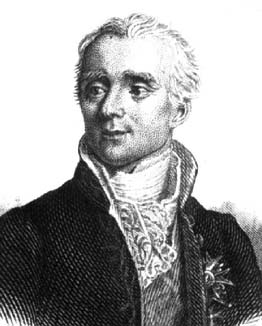
\includegraphics[width=\textwidth]{Laplace}
\end{minipage}
\begin{minipage}{0.6\textwidth}
\begin{center}
  \bf \Large Pierre-Simon Laplace\\
  \normalsize 1749 - 1827
\end{center}
Grondlegger van de kansrekening. Bewees daarnaast ook dat ons zonnestelsel stabiel is. Introduceerde potentiële energie. Leent zijn naam aan de Laplace coëfficiënten.\\

De theorie van de kansrekening is in zijn essentie niets anders dan het gezond verstand herleidt tot analyse. Het maakt het ons mogelijk om exact vast te leggen wat de intuïtie ons reeds vertelt, maar wat we niet aan een ander kunnen verklaren.\\ \hfill{Uit \em Théorie Analytique des Probabilitiés (1812)}
\end{minipage}
\end{mdframed}

\begin{oefening}
In een vaas zitten 20 identieke balletjes met daarop telkens een verschillend getal van 1 tot 20. Beschouw het kansexperiment: 1 balletje uit de vaas nemen.\\
Geef de uitkomstenverzameling $U$:
  \arules{1}
\begin{enumerate}[(a)]
  \item Geef de gebeurtenis $A$ en de kans $P(A)$ dat het getrokken getal negatief is.
  \arules{2}
  \item Geef de gebeurtenis $B$ en de kans $P(B)$ dat het getrokken getal deelbaar door 7 is.
  \arules{2}
  \item Geef de gebeurtenis $C$ en de kans $P(C)$ dat het getrokken getal een priemgetal is.
  \arules{2}
  \item Geef de gebeurtenis $D$ en de kans $P(D)$ dat het getrokken getal $\leq 50$ is.
  \arules{2}
  \item Geef de gebeurtenis $E$ en de kans $P(E)$ dat het getrokken getal een veelvoud van 5 is.
  \arules{2}
  \item Geef de gebeurtenis $F$ en de kans $P(F)$ dat het getrokken getal deelbaar door 14 is.
  \arules{2}
\end{enumerate}
\end{oefening}

\paragraph*{Opmerking}
Laplace zullen we vooral de beperktheid van zijn methode verwijten. Alleen die
experimenten waarvoor we $U$ kunnen herleiden tot een eindige verzameling van
uitkomsten die alle even waarschijnlijk zijn, komen in aanmerking. Als we daarbij
bedenken, dat {\em even waarschijnlijk} afgeleid wordt uit {\em dezelfde kanswaarde}
komen we automatisch in een niet te doorbreken kringloop terecht. Geven we een
concreet tegenvoorbeeld.\\
Beschouwen we het experiment $E$: het voorspellen van de uitslag van een
voetbalwedstrijd met $U = \{t, g, v\}$. ($t$: de thuisploeg wint, $g$: beide ploegen spelen
gelijk, $v$: de ploeg op verplaatsing wint). Hierbij zijn niet alle uitkomsten even
waarschijnlijk. Bovendien speelt de sterkte van de betrokken elftallen een rol. En aan
wat meet men de sterkte? Jawel, aan de hand van de bekomen resultaten. Hier faalt
dus de regel van Laplace. We mogen ze hier dus niet gebruiken.

\subsection{De complementregel}

\subsubsection{Tegengestelde gebeurtenis $\bar{A}$}

\paragraph*{Definitie} $\bar{A}$ is de gebeurtenis: $A$ doet zich {\em niet} voor. We noemen $\bar{A}$ de tegengestelde gebeurtenis van $A$.

\paragraph*{Gevolg}
  \begin{mdframed}
  $$\bar{A}=U\setminus A$$
  \end{mdframed}

Met andere woorden, $\bar{A}$ is het complement van $A$ in $U$.

\paragraph*{Voorbeelden} 
\begin{itemize}
  \item $E_1$: Een muntstuk opgooien. Neem als gebeurtenis $A$: kop gooien\\
  $\bar{A}=\{m\}$, inderdaad $\bar{A}=U\setminus A=\{k,m\}\setminus\{k\}=\{m\}$
  \item $E_2$: Een kaart trekken uit een spel van 52 kaarten. Neem als gebeurtenis $A$: geen aas trekken.\\
  Als $A$ geen aas trekken is, dan is het tegengestelde wel een aas trekken: $\bar{A}=\{a_h, a_r, a_s, a_k\}$. Het is duidelijk dat de tegengestelde gebeurtenis beschrijven eenvoudiger is dan de gebeurtenis zelf.
  \item $E_3$: Verjaren in de maand mei. Neem als gebeurtenis $A$: op een even dag verjaren.\\
  $\bar{A}$ is dan op een oneven dag verjaren, dus $\#\bar{A}=16$ want $\#U=31$ en $\#A=15$.
\end{itemize}

\subsubsection{De kans op tegengestelde gebeurtenissen}

\paragraph*{Stelling} Voor twee tegengestelde gebeurtenissen $A$ en $\bar{A}$ geldt:
$$P(A) + P(\bar{A})=1$$

\paragraph*{Bewijs} Stel de uitkomstenverzameling $U$ met $\#U = n$ en de gebeurtenis $A$ met $\#A = k$ dan
geldt voor de tegengestelde gebeurtenis $\bar{A}$ dat $\#\bar{A} = n - k$.
We berekenen nu met Laplace $P(A)$ en $P(\bar{A})$
\begin{eqnarray*}
  P(A)&=&\dfrac{\#A}{\#U}=\dfrac{k}{n}\\
  P(\bar{A})&=&\dfrac{\#\bar{A}}{\#U}=\dfrac{n-k}{n}=1-\dfrac{k}{n}=1-P(A)\\
\end{eqnarray*}
dus: $P(A)+P(\bar{A})=1$.

\paragraph*{Toepassing}
Het is soms eenvoudiger de kans op de tegengestelde gebeurtenis te berekenen en
daarna voor $P(A)$ de omgevormde formule te gebruiken.\\
\begin{mdframed}
$$P(A)=1-P(\bar{A})$$
\end{mdframed}

We noemen bovenstaande formule de {\bf complementregel} en kan soms handig gebruikt worden in oefeningen. Meestal als het te moeilijk is om de kans op een gebeurtenis te berekenen, dan zal het heel gemakkelijk zijn om de kans op de tegengestelde gebeurtenis te berekenen.

\begin{oefening}
Een zuivere dobbelsteen wordt tweemaal na elkaar lukraak opgegooid. Bereken de
kans om minstens één zes te gooien.
\arules{10}
\end{oefening}

\begin{oefening}
Uit een spel van 52 kaarten trekt men ná elkaar vijf kaarten (met terugleggen). Hoe
groot is de kans op: minstens één aas?
\end{oefening}

\pagebreak

\subsection{Somregel}

\subsubsection{Doorsnede van twee gebeurtenissen $A\cap B$}

\paragraph*{Definitie}
$A\cap B$, $A$ {\bf doorsnede} $B$, is de gebeurtenis: $A$ en $B$ doet zich voor.

\paragraph*{Voorbeeld}
Beschouw experiment $E$, het trekken van een kaart uit een pak van 52 kaarten. Beschouw twee gebeurtenissen, A: een rode kaart trekken, B: een aas trekken. Dan is\\
\begin{eqnarray*}
A\cap B &=& \{2_h, 3_h, \ldots, k_h, a_h, 2_r, 3_r, \ldots, k_r, a_r\}\cap\{a_h, a_s, a_r, a_k\}\\
        &=& \{a_h, a_r\}
\end{eqnarray*}

\subsubsection{Vereniging (unie) van twee gebeurtenissen $A\cup B$}

\paragraph*{Definitie}
$A\cup B$, $A$ {\bf unie} $B$, is de gebeurtenis: $A$ of $B$ doet zich voor.

\paragraph*{Voorbeeld}
Beschouw experiment $E$, het trekken van een kaart uit een pak van 52 kaarten. Beschouw twee gebeurtenissen, A: een harten trekken, B: een koeken trekken. Dan is\\
\begin{eqnarray*}
A\cup B &=& \{2_h, 3_h, \ldots, k_h,a_h\}\cup\{2_r, 3_r, \ldots, k_r, a_r\}\\
        &=& \{2_h, 3_h, \ldots, k_h, a_h, 2_r, 3_r, \ldots, k_r, a_r\}
\end{eqnarray*}

\subsubsection{Elkaar uitsluitende gebeurtenissen}

\paragraph*{Definitie}
We zeggen dat twee gebeurtenissen {\bf elkaar uitsluiten} (disjunct zijn) als hun doorsnede
de onmogelijke gebeurtenis is.\\
\begin{mdframed}
$$A\mbox{ en }B\mbox{ disjunct }\Leftrightarrow A\cap B = \emptyset$$
\end{mdframed}

\paragraph*{Voorbeeld}
Beschouw experiment $E$, het kiezen van een leerling uit de klas. Dan is de gebeurtenis $A$ een jongen kiezen disjunct met de gebeurtenis $B$ een meisje kiezen.

\pagebreak
\begin{samepage}
\subsubsection{De kans op de vereniging van twee gebeurtenissen}

\paragraph*{Stelling }Voor de vereniging van twee willekeurige gebeurtenissen A en B, geldt:\\
\begin{mdframed}
$$P(A \cup B) = P(A) + P(B) - P(A \cap B)$$
\end{mdframed}

\paragraph*{Bewijs}
\begin{center}
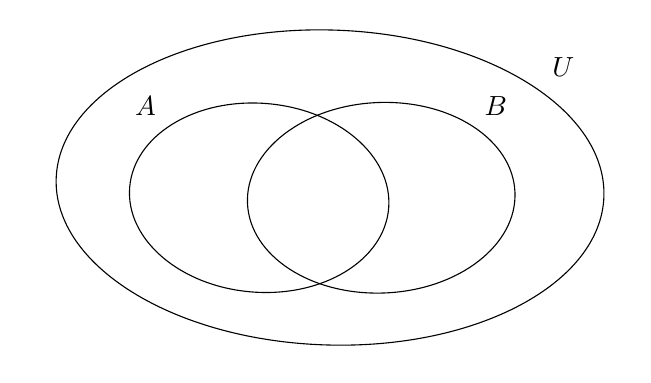
\begin{tikzpicture}[line cap=round,line join=round,>=triangle 45,x=1.0cm,y=1.0cm]
\clip(1.96,0.6) rectangle (9.52,4.75);
\draw [rotate around={-1.89:(5.8,2.72)}] (5.8,2.72) ellipse (3.48cm and 2.0cm);
\draw [rotate around={-4.59:(4.9,2.59)}] (4.9,2.59) ellipse (1.65cm and 1.2cm);
\draw [rotate around={2.41:(6.45,2.59)}] (6.45,2.59) ellipse (1.7cm and 1.21cm);
\draw (8.5,4.5) node[anchor=north west] {$U$};
\draw (3.2,4) node[anchor=north west] {$A$};
\draw (7.64,4) node[anchor=north west] {$B$};
\end{tikzpicture}
\end{center}
Neem $\#U = n$. Op het Venndiagram stel je vast dat: $\#(A\cup B)=\#A + \#B - \#(A\cap B)$. Merk op dat $A \cap B$ een deelverzameling is van zowel $A$ als $B$. We berekenen nu met de regel van Laplace:
\begin{eqnarray*}
  P(A \cup B) &=& \dfrac{\#(A \cup B)}{n}\\
              &=& \dfrac{\#A + \#B - \#(A\cap B)}{n}\\
              &=& \dfrac{\#A}{n} + \dfrac{\#B}{n} - \dfrac{\#(A\cap B)}{n}\\
              &=& P(A) + P(B) - P(A\cap B)
\end{eqnarray*}
\end{samepage}

\begin{oefening}
We gooien lukraak met een zuivere dobbelsteen. Bereken de kans op gebeurtenis C:
een priemgetal of een even getal gooien.
\paragraph*{Oplossing} $\#U=\arule{2cm}$\\
Stel $A$: een priemgetal gooien. $A=\arule{5cm}$\\
Stel $B$: een even getal gooien. $B=\arule{5cm}$\\
Dan is $A\cap B$: een even priemgetal gooien. $A\cap B=\arule{5cm}$\\
Dus $P(C)=P(A\cup B)=$
\arules{2}
\end{oefening}

\begin{oefening}
Uit een spel van 52 kaarten trekken we lukraak een kaart. Hoe groot is de kans dat de
getrokken kaart een harten of een boer is?
\end{oefening}

\subsubsection{Bijzonder geval, de somregel}
Beschouwen we nu twee disjuncte gebeurtenissen $A$ en $B$, dan is $A \cap B = \emptyset$.
De aangepaste formule wordt dan:\\
\begin{mdframed}
$$A \cap B = \emptyset \Rightarrow P(A\cup B)=P(A)+P(B)$$
\end{mdframed}
Deze wet wordt heel dikwijls de {\bf somregel} voor de kansrekening genoemd. Deze wet
kan men uitbreiden voor meerdere gebeurtenissen, maar ze moeten dan wel 2 aan 2
disjunct zijn. We zullen hier niet over uitweiden.

\begin{oefening}
In een urne bevinden zich 8 rode, 5 zwarte en 17 gele bollen. We trekken lukraak een
bol. Bereken de kans dat de bol rood of zwart is.
\arules{9}
\end{oefening}

\subsection{Oefeningen}

\begin{oefening}
Bereken de kans om met een zuivere dobbelsteen
\begin{enumerate}[(a)]
  \item Ten minste 4 ogen te gooien.
  \item Een aantal ogen te gooien dat deelbaar is door 3.
\end{enumerate}
\end{oefening}

\begin{oefening}
Bij het opgooien van een muntstuk zijn er twee even waarschijnlijke uitkomsten: Kop en Munt. Een zuiver muntstuk wordt driemaal opgegooid.
\begin{enumerate}[(a)]
  \item Teken het boomdiagram dat hierbij hoort.
  \item Lees eruit af hoe groot de kans is om precies tweemaal kop te krijgen.
\end{enumerate}
\end{oefening}

\begin{oefening}
In een bak zitten 3 witte, 4 rode en 5 blauwe knikkers. We nemen lukraak 1 knikker. Bereken de kans dat de knikker 
\begin{enumerate}[(a)]
  \item Wit is
  \item Rood is
  \item Blauw is
  \item Wit of rood is
  \item Rood of blauw is
  \item Blauw of wit is
  \item Niet blauw is.
\end{enumerate}
\end{oefening}

\begin{oefening}
In een bak zitten 4 rode en 5 witte knikkers. Men trekt er willekeurig 2 knikkers uit. Bereken de kans
\begin{enumerate}[(a)]
  \item Om 2 knikkers van dezelfde kleur te hebben.
  \item Om precies één rode knikker te hebben.
\end{enumerate}
\end{oefening}

\begin{oefening}
Uit een spel van 52 kaarten trekt men willekeurig één kaart. Bereken de kans
\begin{enumerate}[(a)]
  \item Dat het een 10 is.
  \item Dat het een klaver is.
  \item Dat het een heer, dame of boer is.
  \item Dat het een rode kaart is.
  \item Dat het een aas is.
\end{enumerate}
\end{oefening}

\begin{oefening}
Uit een spel van 32 kaarten (2, 3, 4, 5 en 6 zijn weggenomen) trekt men op aselecte wijze en tegelijkertijd 3 kaarten. Bereken de kans dat
\begin{enumerate}[(a)]
  \item Het drie azen zijn.
  \item Er precies één aas bij is.
  \item Er precies 1 heer en 1 dame bij is.
\end{enumerate}
\end{oefening}

\begin{oefening}
In een klas van 25 leerlingen zijn er 10 die graag dansen en 5 die graag
zingen. Daarbij zijn er 2 leerlingen die zowel graag dansen als zingen. Als we lukraak een
leerling aanduiden, wat is de kans dat die graag danst of graag zingt.
\end{oefening}

\begin{oefening}
Men gooit lukraak drie dobbelstenen op. Wat is de kans dat de som van
het aantal ogen ten minste gelijk is aan 5.
\end{oefening}

\begin{oefening}
Uit een spel van 52 kaarten trek je lukraak vier kaarten. Wat is de kans
dat er precies één boer bij is?
\end{oefening}

\begin{oefening}
Bij een spelletje poker krijgt een speler 5 kaarten uit een spel van 52
kaarten. Bereken voor deze speler de kans dat hij 5 kaarten krijgt van dezelfde kleur.
\end{oefening}

\begin{oefening}
A en B zijn 2 gebeurtenissen bij een kansexperiment waarvoor geldt dat $P(A\bigcup B)=\frac{5}{9}$, $P(\bar{A})=\frac{5}{9}$ en $P(A\bigcap B)=\frac{1}{9}$. Bereken
\begin{exlist}{3}
  \item $P(A)$
  \item $P(B)$
  \item $P(A\setminus B)$
\end{exlist}
\end{oefening}

\begin{oefening}
Uit een spel van 52 kaarten trekken we lukraak een kaart. Bereken de kans dat het geen getal is (dus boer, koningin of koning)  is.
\end{oefening}

\begin{oefening}
Men gooit lukraak drie dobbelstenen op. Wat is de kans dat de som van het aantal ogen ten minste gelijk is aan 5.
\end{oefening}

\begin{oefening}*
Een vaas bevat 3 rode en 2 witte knikkers, een tweede vaas 4 rode en 1 witte. Als men met een dobbelsteen een zes werpt neemt men een knikker uit vaas 2, in alle andere gevallen uit vaas 1. Hoe groot is de kans een witte knikker uit vaas 1 te trekken? 
\end{oefening}

\begin{oefening}*
In een schroevenfabriek fabriceren de machines A, B en C resp. 25, 35 en 40 \% van de totale productie. Van hun producten zijn er resp. 5, 4 en 2 \% defect. Men kiest willekeurig een schroef en deze is slecht. Hoe groot is de kans dat deze gemaakt
is door A, B of C?
\end{oefening}

\pagebreak
\section{Voorwaardelijke kansen}

\subsection{Inleiding}

Beschouw het volgende voorbeeld:

{\em Een medisch team heeft een onderzoek gedaan over het optreden van kleurenblindheid in een bepaalde bevolkingsgroep van 1000 mensen. Hierbij heeft men twee zaken geregistreerd: het geslacht en het al of niet kleurenblind zijn.}

We krijgen de volgende data terug (mannen ($M$), vrouwen ($V$), kleurenblind ($K$), niet kleurenblind ($NK$)):

\begin{center}
  \begin{tabular}{c|c|c|c}
         &  $K$ &  $NK$ & Totaal\\
  \hline
  $M$      & 32 & 368 & 400\\
  $V$      &  6 & 594 & 600\\
  \hline
  Totaal & 38 & 962 & 1000
  \end{tabular}
\end{center}

\begin{oefening}
Bepaal volgende kansen:
\begin{enumerate}[(a)]
  \item $V$: De gekozen persoon is een vrouw\\$\Rightarrow$ $P(V)=\arule{2cm}$
  \item $K$: De gekozen persoon is kleurenblind\\$\Rightarrow$ $P(K)=\arule{2cm}$
  \item $V\cap K$: De gekozen persoon is een vrouw en is kleurenblind\\$\Rightarrow$ $P(V\cap K)=\arule{2cm}$
\end{enumerate}
\end{oefening}

\paragraph*{Opmerking} In de vorige oefening zijn telkens alle experimenten betrokken!


Veronderstel nu dat we zeker weten dat de proefpersoon een vrouw is. We moeten dan enkel nog kijken naar de relevante data, dus enkel bij de rij van de vrouwen. Wat is dan de kans dat ze kleurenblind is? Hiervoor voeren we een nieuwe notatie in:
$$K|V:\mbox{De gekozen persoon is kleurenblind, op voorwaarde dat het een vrouw is}$$
$$\Rightarrow\quad P(K|V)=\dfrac{6}{600}=\dfrac{1}{100}$$

\paragraph*{Opmerking} Bij een voorwaardelijke kans is slechts een deel van de experimenten betrokken!

\begin{oefening}
Bereken het product $P(V)\cdot P(K|V)=\arule{3cm}$\\
Wat kan je besluiten?
\arules{3}
\end{oefening}

\begin{oefening}
Bereken $P(K\cap M)$; $P(K|M)$; $P(M)$ en ga na of het product $P(K\cap M)=P(M)\cdot P(K|M)$ ook klopt.
\end{oefening}

\begin{oefening}
Bereken $P(NK\cap M)$; $P(NK|M)$; $P(M)$ en ga na of het product $P(NK\cap M)=P(M)\cdot P(NK|M)$ ook klopt.
\end{oefening}

\subsection{Definitie}

\paragraph*{Definitie}
In de uitkomstenverzameling $U$ onderscheiden we twee gebeurtenissen $A$ en $B$, waarvan $A$ niet onmogelijk is. De {\bf voorwaardelijke kans} op $B$, vooropgesteld dat $A$ zich voordoet, wordt gegeven door\\
\begin{mdframed}
$$P(B|A)=\dfrac{P(A\cap B)}{P(A)}\qquad\mbox{ met }P(A)\neq 0\;.$$
\end{mdframed}

\paragraph*{Definitie}
Voorgaande formule kan ook geschreven worden in de vorm
$$P(A\cap B)=P(B|A)\cdot P(A)$$
en we spreken dan van de {\bf productregel}.

\paragraph*{Definitie} Een kans waarop geen voorwaarde wordt gesteld zullen we een {\bf gewone kans} noemen.

\begin{oefening}
Zeg telkens om welke kans het gaat en bereken de kans:
\begin{enumerate}[(a)]
  \item $P(M\cap K)=$\arulefill
  \arules{1}
  \item $P(M|K)=$\arulefill
  \arules{1}
  \item $P(K|M)=$\arulefill
  \arules{1}
\end{enumerate}
\end{oefening}

\begin{oefening}
Uit de 20 nummers $\{1,2,3,\ldots,20\}$ trek je er één. Als je 3, 5, 6, 11 of 18 trekt heb je
prijs. Bereken de kans op volgende gebeurtenissen:
\begin{enumerate}[(a)]
  \item $A$: je hebt prijs.
  \item $B$: je hebt prijs, vooropgesteld dat het nummer even is.
  \item $C$: je hebt prijs, vooropgesteld dat het nummer een 4-voud is.
  \item $D$: het getrokken nummer is priem, vooropgesteld dat je prijs hebt.
\end{enumerate}
\end{oefening}

\subsection{Eigenschappen}

\paragraph*{Eigenschap} De voorwaardelijke kans is ook {\bf een kans}.

Dus er geldt ook
$$0\leq P(B|A)\leq 1$$

\paragraph*{Eigenschap} $U|A$ is de zekere gebeurtenis.

Want:
\begin{eqnarray*}
  P(U|A) &=& \dfrac{P(U\cap A)}{P(A)}\\
         &=& \dfrac{P(A)}{P(A)}\\
         &=& 1
\end{eqnarray*}

\paragraph*{Stelling} Somregel voor voorwaardelijke kansen kan bewezen worden
$$B\cap C=\emptyset \Rightarrow P((B\cup C)|A)=P(B|A)+P(C|A)$$

\begin{oefening}*
Bewijs voorgaande stelling.
\end{oefening}

\begin{oefening}*
Stel $U=\{1,2,3,4\}$. Beschouw de gebeurtenissen $A=\{1\}$, $B=\{2\}$ en $C=\{1,4\}$. Bepaal $P((A\cap B)|C)$.
\end{oefening}

\subsection{Oefeningen}

\begin{oefening}
Men werpt met een zwarte en een witte dobbelsteen. Stel de gebeurtenissen:
\begin{itemize}
  \item $A$: De witte dobbelsteen valt op 3.
	\item $B$: De som van het aantal ogen is even.
\end{itemize}
Bereken $P(A)$, $P(B)$, $P(A|B)$ en $P(B|A)$.
\end{oefening}

\begin{oefening}
Je ontmoet een dochter van een gezin met twee kinderen. Hoe groot is de kans dat ook het andere kind een meisje is?
\end{oefening}

\begin{oefening} % Bron: wwwhome.cs.utwente.nl/~meijertmj/
Uit statistische gegevens met betrekking tot fietsendiefstallen is het volgende af te leiden.
\begin{itemize}
  \item Van de gestolen fietsen is 40\% verzekerd
  \item Bij diefstal van een fiets wordt in 72\% van de gevallen aangifte gedaan.
  \item Bij diefstal van een verzekerde fiets wordt in 90\% van de gevallen aangifte gedaan.
\end{itemize}
\begin{enumerate}[(a)]
  \item Op de vraag hoe groot de kans is dat een (willekeurige) gestolen fiets verzekerd is en er aangifte wordt gedaan van diefstal, antwoordt Gilles $0.90\times0.40 = 36\%$ en Emma $0.72\times0.40 = 28.8\%$. Wie heeft er gelijk? 
  \item Bereken de kans dat een fiets, waarvan de eigenaar aangifte doet van diefstal, verzekerd is.
\end{enumerate}
\end{oefening}

\begin{oefening}
We gooien met een eerlijke dobbelsteen. Bepaal de kans om minder dan vier ogen te gooien gegeven dat er een even aantal ogen gegooid werd.
\end{oefening}

\begin{oefening} % Bron: wwwhome.cs.utwente.nl/~meijertmj/
ELISA-tests worden gebruikt om donor-bloed te onderzoeken op aanwezigheid van het AIDS-virus. De test detecteert in feite antilichamen, stoffen die door het lichaam worden geproduceerd wanneer het virus aanwezig is. Als er antilichamen zijn, is ELISA positief met kans 0.997 en negatief met kans 0.003. Indien het onderzochte bloed niet met AIDS-antilichamen is besmet, is de kans dat ELISA een positief resultaat geeft gelijk aan 0.015, en de kans dat er een negatief resultaat komt is 0.985. (Omdat ELISA tot doel heeft het AIDS-virus buiten de bloedbanken te houden, is de betrekkelijk grote kans (0.015) op een foutief positief antwoord acceptabel, tegenover de geringe kans (0.003) op het niet herkennen van besmet bloed. Deze kansen zijn afhankelijk van de deskundigheid van het laboratorium dat de tests uitvoert.) Veronderstel dat 1\% van een grote populatie de AIDS-antilichamen in het bloed heeft.
\begin{enumerate}[(a)]
  \item Bereken de kans dat ELISA voor een aselect gekozen persoon uit deze populatie een positief resultaat laat zien.
  \item Bereken de kans dat iemand de antilichamen heeft, gegeven dat ELISA positief was.
\end{enumerate}
{\em (Deze opgave illustreert een feit dat belangrijk wordt wanneer men overweegt voorstellen te doen voor grootschalig testen op AIDS of illegale drugs: als het verschijnsel waarop getest wordt in de populatie ongewoon is, zullen de meeste positieve uitkomsten foutief zijn, zelfs als de test een zeer grote kans heeft om per geval een corrcet resultaat te geven.)}
\end{oefening}

\begin{oefening}
In een zak zitten 6 blauwe en 3 gele ballen. Alle ballen hebben een gelijke kans om getrokken te worden en elke bal die getrokken wordt, moet je onmiddellijk terug in de zak leggen.
\begin{enumerate}[(a)]
  \item Je trekt een bal uit de zak. Formuleer een zo gedetailleerd mogelijke uitkomstenverzameling.
  \item Je trekt 4 ballen uit de zak. Formuleer een zo gedetailleerd mogelijke uitkomstenverzameling.
  \item Je trekt twee ballen uit de zak. Wat is de kans dat ze allebei blauw zijn?
  \item Je trekt drie keer een bal. Wat is de kans dat de tweede bal geel is?
  \item Je trekt drie keer een bal. Wat is de kans dat de je juist één blauwe bal trekt?
  \item Wat is de kans dat je bij het trekken van 3 ballen minstens één blauwe bal uit de zak haalt?
  \item Wat is de kans om bij drie trekkingen twee ballen van een verschillende kleur uit de zak te halen?
  \item Je trekt 3 ballen. Gegeven dat er minstens één blauwe bij is, wat is de kans dat de andere 2 geel zijn?
\end{enumerate}
\end{oefening}

\begin{oefening}
Een familie heeft drie kinderen die we rangschikken in volgorde van geboorte $(X_1, X_2, X_3)$. $X_i$ kan de waarde $M$ of $J$ aannemen, naargelang het $i$-de geboren kind een jongen of een meisje is. Veronderstel dat de kans op een jongen en een meisje dezelfde is en dat opeenvolgende geboortes elkaar niet beïnvloeden. Wat is de kans dat er twee meisjes zijn, gegeven:
\begin{enumerate}[(a)]
  \item dat er minstens één jongen is, of
  \item de oudste van de drie zeker een jongen is.
\end{enumerate}
\end{oefening}

\begin{oefening}
Toon aan dat uit $P(A|B)=P(A)$ volgt dat $P(B|A)=P(B)$, voor twee gebeurtenissen $A$ en $B$ met niet nul kansen.
\end{oefening}

\begin{oefening}
Een dronken bestuurder pleegt 10 maal zoveel vluchtmisdrijf als een nuchtere bestuurder. Iemand pleegt een vluchtmisdrijf. Wat is de kans dat hij dronken was, als je weet dat 1 op 50 autobestuurders dronken is.
\end{oefening}

\pagebreak
\section{Statistisch (on)afhankelijke gebeurtenissen}

\subsection{Definitie onafhankelijke gebeurtenissen}

We veronderstellen dat $A$ en $B$ gebeurtenissen zijn horende bij een experiment $E$ met uitkomstenverzameling $U$ en dat $P(A)\cdot P(B) \neq 0$. Dan definiëren we
$$A \mbox{ {\bf onafhankelijk} van } B \Leftrightarrow P(A)=P(A|B)$$

\paragraph*{Eigenschap 1} $A$ onafhankelijk van $B \Leftrightarrow B$ onafhankelijk van $A$

\paragraph*{Eigenschap 2} $A$ onafhankelijk van $B \Leftrightarrow P(A\cap B)=P(A)\cdot P(B)$

\begin{oefening}
Bewijs eigenschap 2.
\arules{6}
\end{oefening}

Voorgaande eigenschap kan men nu ook gaan beschouwen als een nieuwe definitie voor twee onafhankelike gebeurtenissen. M.a.w.:

\paragraph*{Definitie}
\begin{mdframed}
$$A \mbox{ {\bf onafhankelijk} van } B \Leftrightarrow P(A\cap B)=P(A)\cdot P(B)$$
\end{mdframed}

\subsection{Definitie afhankelijke gebeurtenissen}

 Men zal dan ook dikwijls zeggen dat 2 gebeurtenissen afhankelijk zijn als en slechts als de gelijkheid niet waar is:

\paragraph*{Definitie}
\begin{mdframed}
$$A \mbox{ {\bf afhankelijk} van } B \Leftrightarrow P(A\cap B)\neq P(A)\cdot P(B)$$
\end{mdframed}

\begin{oefening} We kiezen willekeurig een getal van $1$ tot $12$. Daarbij beschouwen de volgende gebeurtenissen: $A$, het getal is even en $B$, het getal is een drievoud. Onderzoek de (on)afhankelijkheid van $A$ en $B$.\\
$U=\{\arule{8cm}\}$ met $\#U=\arule{2cm}$\\
$A=\{\arule{8cm}\}$ met $\#A=\arule{2cm}$\\
$B=\{\arule{8cm}\}$ met $\#B=\arule{2cm}$\\

$A\cap B=\{\arule{4cm}\}$ met $\#(A\cap B)=\arule{2cm}$\\

$\Rightarrow P(A)=\arule{2cm}, P(B)=\arule{2cm}, P(A\cap B)=\arule{2cm}$\\

En dus $A$ en $B$ zijn \arule{4cm} want \arule{4cm}
\end{oefening}

\begin{oefening}
We kiezen willekeurig een getal uit $\{1,2,\ldots, 9\}$. Daarbij beschouwen de volgende gebeurtenissen: $A$, het getal is even en $B$, het getal is een drievoud. Onderzoek de (on)afhankelijkheid van $A$ en $B$.
\end{oefening}

\subsection{Productwetten}

We kunnen nu voorgaande definities en eigenschappen samennemen om de zogenaamde productwetten voor de samengestelde gebeurtenis $A\cap B$ op te stellen:\\

\begin{mdframed}\vspace*{-0.5cm}
\begin{eqnarray*}
  P(A\cap B) &=& P(A)\cdot P(B|A) \mbox{ met } P(A)\neq 0\\
             &=& P(B)\cdot P(A|B) \mbox{ met } P(B)\neq 0\\
             &=& P(B)\cdot P(A) \mbox{ met $A$ en $B$ onafhankelijk}
\end{eqnarray*}
\end{mdframed}

Deze stellen ons in staat om gemakkelijk de kans op een samengestelde beslissing $P(A\cap B)$ te berekenen, de eerste twee formules wanneer de ene gebeurtenis de andere beïnvloed (gebeurtenissen afhankelijk) en de laatste formule wanneer de gebeurtenissen elkaar niet beïnvloeden (gebeurtenissen onafhankelijk).

Dit wordt meestal gebruikt als we besluiten moeten trekken over de kanswaarde van een trekking met en zonder terugleggen, zoals bijvoorbeeld in de volgende oefeningen:

\begin{oefening}
In een vaas zitten 3 gele, 5 rode en 10 groene bollen. Jan trekt eerst een bol, legt deze terug en daarna trekt Karel een bol. Bereken de kans op: Jan trekt een rode bol en Karel trekt een groene bol.

Definieer de gebeurtenissen:
\begin{itemize}
  \itemsep0.1em
  \item $J_{rood}$: Jan trekt een rode bol.
  \item $K_{groen}$: \arulefill
\end{itemize}
\vspace*{0.5cm}
We wensen dus de kans $P(J_{rood}\cap K_{groen})$ te berekenen:\\
$J_{rood}$ en $K_{groen}$ zijn \verb#afhankelijk#/\verb#onafhankelijk#.\\
We gebruiken dus de formule:
$\arule{10cm}$\\
We berekenen:
$$P(J_{rood})=\arule{4cm} \qquad\mbox{ en }\qquad P(K_{groen})=\arule{4cm}$$
Besluit:
$$\arule{10cm}$$
\end{oefening}

\begin{oefening}
In een vaas zitten 3 gele, 5 rode en 10 groene bollen. Jan trekt eerst een bol, legt deze {\em niet} terug en daarna trekt Karel een bol. Bereken de kans op: Jan trekt een rode bol en Karel trekt een groene bol.

Definieer de gebeurtenissen:
\begin{itemize}
  \itemsep0.1em
  \item $J_{rood}$: Jan trekt een rode bol.
  \item $K_{groen}$: \arulefill
\end{itemize}
\vspace*{0.5cm}
We wensen dus de kans $P(J_{rood}\cap K_{groen})$ te berekenen:\\
$J_{rood}$ en $K_{groen}$ zijn \verb#afhankelijk#/\verb#onafhankelijk#.\\
We gebruiken dus de formule:
$$\arule{10cm}$$
Als we dus mogen veronderstellen dat Jan een rode bol heeft getrokken, hoeveel groene bollen kan Karel dan nog trekken? \arule{2cm}
Dus:
$$P(K_{groen}|J_{rood})=\arule{4cm}$$
Besluit:
$$\arule{10cm}$$
\end{oefening}

\paragraph*{Opmerking}

Aangezien $P(A\cap B\cap C)=P(A)\cdot P(B|A) \cdot P(C|(A\cap B))$, ligt de uitbreiding van de formule naar 3 verzamelingen niet voor de hand! We zullen bijgevolg geen kansen berekenen waarbij de doorsnede van meer dan 2 afhankelijke gebeurtenissen wordt gevraagd. Het geval waarbij de verschillende gebeurtenissen onafhankelijk, bijvoorbeeld een trekking met teruglegging die steeds herhaald wordt, is kan wel gemakkelijk veralgemeend worden.

\begin{oefening}
Maak deze veralgemening:\\
$A$, $B$ en $C$ zijn paarsgewijze onafhankelijk, dan geldt $$P(A\cap B\cap C)=\arule{6cm}$$
\end{oefening}

\subsection{Herhaalde experimenten}

Stel dat we een experiment $E$ $n$ keer herhalen. Hoe groot is de kans dat de gebeurtenis $A$ zich telkens voordoet?
Laten we dit probleem met een voorbeeld verduidelijken.


\paragraph*{Voorbeeld}
Stel $E$ is het experiment waarbij we een kaart trekken uit een spel van 52 speelkaarten met terugleggen en $A$ is de gebeurtenis waarbij we een schoppen trekken.
Hoe groot is de kans dat we bij $n$ trekkingen telkens een schoppen trekken?

We noemen 
\begin{center}
  \renewcommand{\arraystretch}{1}
  \begin{tabular}{r@{ }c@{ }c@{ }c@{ }c@{ }c}
    $A_1$: & De gebeurtenis & $A$ & doet zich de & eerste maal & voor\\
    $A_2$: &        "       & $A$ &       "      & tweede maal &   " \\
    $A_3$: &        "       & $A$ &       "      & derde maal &   " \\
    \vdots &    \vdots      & \vdots &  \vdots   &  \vdots  &\vdots \\
    $A_n$: &        "       & $A$ &       "      & n-de maal &   " \\
  \end{tabular}
\end{center}

Met behulp van Laplace vinden we de kansen op elk van de gebeurtenissen:
$$P(A_1)=P(A_2)=P(A_3)=\cdots=P(A_n)=P(A)=p$$

Dan is:
\begin{align*}
  P(A_1\cap A_2 \cap A_3\cap \cdots \cap A_n)&=P(A_1)\cdot P(A_2)\cdot P(A_3)\cdot \cdots \cdot P(A_n)\\
                                             &=p\cdot p\cdot p\cdot \cdots \cdot p\\
                                             &= p^n
\end{align*}
In ons voorbeeld is $p=\dfrac{13}{52}=\dfrac{1}{4}$. De kans om dus vijf keer na elkaar schoppen te bekomen is dus:
$$P(A_1\cap A_2 \cap A_3\cap A_4 \cap A_5)=\left(\dfrac{1}{4}\right)^5=\dfrac{1}{1024}\;.$$

%\newpage
\paragraph*{Uitbreiding} We kunnen dit op een voor de hand liggende manier uitbreiden naar een experiment $E$ dat we $n$ keer herhalen, maar waarbij we willen weten wat de kans is om $n$ verschillende gebeurtenissen na elkaar waar te nemen. Met andere woorden, hoe groot is de kans dat de gebeurtenis $A_1$ zich de eerste keer voordoet, de gebeurtenis $B_2$ zich de tweede keer voordoet, \ldots?
$$P(\underbrace{A_1\cap B_2\cap\cdots}_{n\mbox{ \scriptsize gebeurtenissen}})=\underbrace{P(A_1)\cdot P(B_2)\cdot \cdots}_{n\mbox{ \scriptsize factoren}}$$

\begin{oefening}
In een vaas zitten 3 rode, 5 gele en 10 groene bollen. Je trekt drie keer na elkaar een bol en legt hem telkens terug. Bereken de kans dat je eerst een rode dan een groene en tenslotte opnieuw een rode bol trekt.

Veronderstel de volgende gebeurtenissen:
\begin{itemize}
  \itemsep0.2em
  \item $R_1$: De eerste bol is rood.
  \item $G_2$: \arulefill
  \item $R_3$: \arulefill
\end{itemize}
\vspace*{0.1cm}
\arules{4}
\end{oefening}

\begin{oefening}*
In een vaas zitten 3 rode, 5 gele en 10 groene bollen. Je trekt drie keer na elkaar een bol en legt hem niet terug. Bereken de kans dat je eerst een rode dan een groene en tenslotte opnieuw een rode bol trekt.
\end{oefening}

\subsection{Oefeningen}

\begin{oefening}
Een vaas $V_1$ bevat 2 zwarte en 3 witte bolletjes. Een andere vaas $V_2$ bevat er 4 zwarte
en 5 witte. Men neemt willekeurig een bolletje uit vaas $V_1$ en werpt dit in $V_2$. Men
trekt daarna een bolletje uit $V_2$ en dit blijkt zwart te zijn. Bereken de kans dat er een
wit bolletje werd verwisseld van vaas.
\end{oefening}

\begin{oefening}
In een gezin zijn er $n$ kinderen. Stel de gebeurtenissen:
\begin{itemize}
  \item $A$: Het gezin telt kinderen van beide sekse.
  \item $B$: Het gezin telt ten hoogste één meisje.
\end{itemize}
	Onderzoek de (on)afhankelijkheid van A en B als:
\begin{enumerate}[(a)]
  \item Het gezin 2 kinderen telt ($n = 2$)
  \item Het gezin 3 kinderen telt ($n = 3$)
\end{enumerate}
\end{oefening}

\begin{oefening}*
Als $\{B,C\}$ een partitie is van $U$, bewijs dan dat voor elke deelverzameling $A\subset U$ geldt dat
$$P(A)=P(B)\cdot P(A|B)+P(C)\cdot P(A|C)\;.$$
\end{oefening}

\begin{oefening}
Een lot bevat 60 rode en 40 blauwe lampen. De kans dat een rode lamp kapot is bedraagt $\dfrac{1}{14}$. De kans dat een blauwe lamp kapot is bedraagt $\dfrac{2}{35}$. We trekken lukraak een lamp. Hoe groot is de kans op een goede lamp?
\end{oefening}

\newpage
\appendix
\section*{Bijlagen}

\subsection*{Het kaartspel}
Het kaartspel bestaat uit 4 soorten: klaveren (k), ruiten (r), harten (h) en schoppen (s). De soorten worden verder onderverdeeld in 13 kaarten: 2, 3, 4, 5, 6, 7, 8, 9, 10, boer (j), koningin (q) en koning (k), aas (a). Er zijn ook twee soorten kleuren, de klaveren en de schoppen zijn zwart, de ruiten en harten zijn rood. De jokers negeren wij. Als we over een kaart spreken, dan schrijven we eerst de volgorde en dan als index de soort. Zo wordt de harten dame $q_h$ en de schoppen zeven $7_s$.

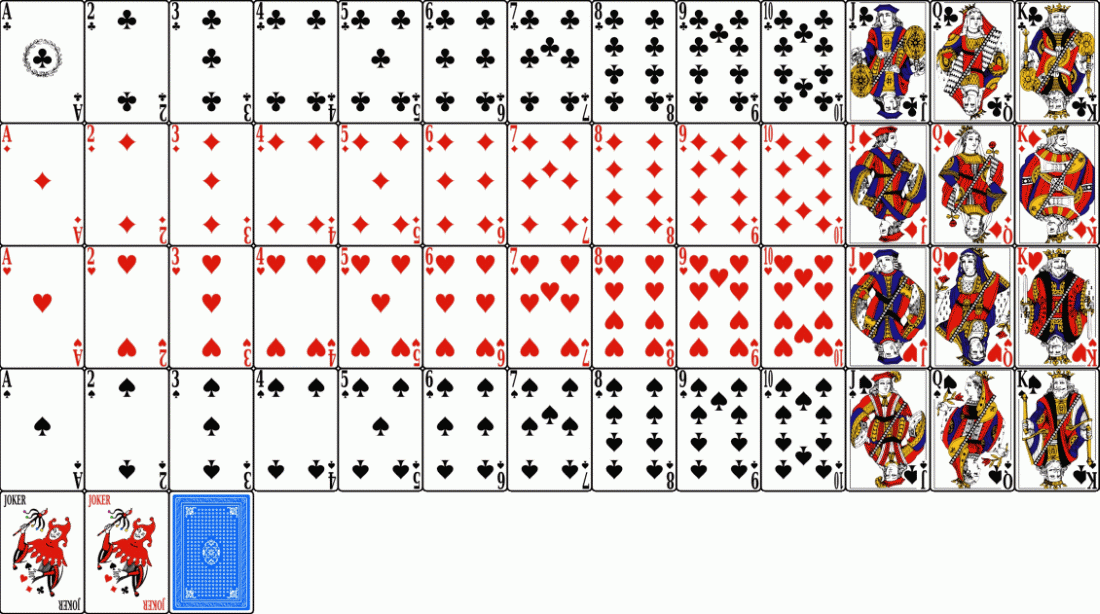
\includegraphics[width=\textwidth, angle=0]{kaartspel}


%%%%%%%%%%%%%%%%%%%%%%%%%%%%%%%%%%%%%%%%%%%%%%%%%%%%%%%%%%%%%%%%%%%%%%
\end{document}



\begin{minipage}[c]{0.4\textwidth}
\end{minipage}
\begin{minipage}[c]{0.6\textwidth}
\dotlines{10}
\end{minipage}




















